%=========================================================
\chapter{Modelo de comportamiento del subsistema: Gestión de proyectos}
\label{cap:reqSist}

En ese capítulo se describen los casos de uso referentes a la gestión de proyectos y a la configuración del proyecto.

%---------------------------------------------------------

\begin{shaded}
		\textcolor{NavyBlue}{\Large\textbf{Elementos de un caso de uso}}
		\begin{itemize}
			\item \textbf{Resumen:} Descrpción textual del caso de uso
			\item \textbf{Actores:} Lista de los que  intervienen en el caso de uso.
			\item \textbf{Propósito:} Una breve descripción del objetivo que busca e actor al ejecutare el caso de uso.
			\item \textbf{Entradas:} Lista de los datos requeridos durante a ejecución del caso de uso.
			\item \textbf{Salidas:} Lista de los datos de salida que presetan al sistema durante la ejecuciń del caso de uso.
			\item \textbf{Precondiciones:} Descrpción de las operaciones o condiciones que se deben cumplir previamente para el caso de uso pueda ejecutarse correctamente.
			\item \textbf{Postcondiciones:} Lista de los cambios que ocurrirán en el sistema después de la ejecución del caso de uso y de las consecuencias del sistema.
			\item \textbf{Reglase de negocio:} Lista de las reglas que describen, limitan o controlan algún aspecto del negocio del caso de uso.
			\item \textbf{Errores:} Lista de los posibles errores que pueden surgir surante la ejecución del caso de uso.
			\item \textbf{Trayectoria:} Secuencia de los pasos que ejecutará el caso de uso
		\end{itemize}		
	\end{shaded}
\newpage

%----------------------------------------------------------------------------
% \IUref{IUAdmPS}{Administrar Planta de Selección}
% \IUref{IUModPS}{Modificar Planta de Selección}
% \IUref{IUEliPS}{Eliminar Planta de Selección}

% 


% Copie este bloque por cada caso de uso:
%-------------------------------------- COMIENZA descripción del caso de uso.

%\begin{UseCase}[archivo de imágen]{UCX}{Nombre del Caso de uso}{
%--------------------------------------
	\begin{UseCase}{CU03}{Crear Proyecto}{
		Permite a un usuario la creación de un nuevo proyecto
	}
		\UCitem{Actor}{\hyperlink{Líder de proyecto}{Líder de proyecto}}
		\UCitem{Propósito}{Crear un proyecto.}
		\UCitem{Entradas}{\begin{itemize}
		\item Líder de proyecto: Lo obtiene el sistema
		\item Nombre: Se ingresa desde el teclado
		\item Fecha de inicio: Se selecciona de un calendario
		\item Fecha de térmico: Se selecciona de un calendario
		\item Descripción: Se ingresa desde el teclado

		\end{itemize}
.}
		\UCitem{Salidas}{Proyecto registrado: Lo genera el sistema .}
		\UCitem{Destino}{Pantalla de listado de proyectos}
		\UCitem{Precondiciones}{Haber iniciado sesión}
		\UCitem{Postcondiciones}{El proyecto queda registrado en el sistema}
		\UCitem{Errores}{La fecha de término es anterior a la fecha de inicio
}
		\UCitem{Observaciones}{}
	\end{UseCase}
%--------------------------------------
	\begin{UCtrayectoria}{Principal}
		\UCpaso[\UCactor] Da click en el menú de proyectos.
		\UCpaso[\UCactor]Da click en el botón registrar proyecto.
       	\UCpaso Muestra la pantalla de registrar proyecto.\label{Crear}
        \UCpaso[\UCactor] Ingresa el nombre, fecha de inicio, fecha de término y descripción.  \Trayref{A}
        \UCpaso Verifica que la fecha de inicio sea anterior a la fecha de fin. \Trayref{B}
       \UCpaso  Muestra la pantalla de mis proyectos
	\end{UCtrayectoria}

%--------------------------------------		
		\begin{UCtrayectoriaA}{A}{ El actor no ingreso los datos requeridos}
			\UCpaso Muestra mensaje de falta de datos requeridos
			\UCpaso Continua en el paso \ref{Crear} del \UCref{CU03}.
		\end{UCtrayectoriaA}
%--------------------------------------		
		\begin{UCtrayectoriaA}{B}{ El actor ingresó una fecha de inicio inválida}
			\UCpaso Muestra mensaje de que las fechas no son válidas.
			\UCpaso Continua en el paso \ref{Crear} del \UCref{CU03}.
		\end{UCtrayectoriaA}
		
		
%-------------------------------------- TERMINA descripción del caso de uso.
%======================================================================================
\begin{UseCase}{CU16}{Editar Proyecto}{
		Permite al Lider de proyecto modificar los parametros de información del proyecto.
	}
		\UCitem{Actor}{\hyperlink{LiderProyecto}{Lider de proyecto}}
		\UCitem{Propósito}{Permitír al Lider de proyecto modificar la información de coniguración del proyecto}
		\UCitem{Entradas}{\begin{itemize}
		\item Nombre: se ingresa desde teclado
		\item Fecha de inicio: Se ingresa desde el teclado
		\item Fecha de termino: Se ingresa desde el teclado 
		\end{itemize}
.}
		\UCitem{Salidas}{Proyecto: modificacion de los parametros de cnfiguración del proyecto.}
		\UCitem{Destino}{Pantalla de gestión de proyectos}
		\UCitem{Precondiciones}{Que el proyecto no este finalizado}
		\UCitem{Postcondiciones}{La configuracion del proyecto sera modificada}
		\UCitem{Errores}{}
		\UCitem{Observaciones}{}
	\end{UseCase}
%--------------------------------------
	\begin{UCtrayectoria}{Principal}
		\UCpaso[\UCactor] Da click en el icono 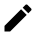
\includegraphics[height=10pt]{./images/iconos/ic_create_black_18dp.png}
        \UCpaso [\UCsist] accede a la pantalla \hyperref[fig:IU16]{IU16 Editar Proyecto}. \label{item:CU16Item1}
		\UCpaso[\UCactor] ingresa los datos en los campos correspondientes. 
      \UCpaso[\UCactor]   solicita el cambio de su contraseña oprimiendo el botón aceptar.
		\UCpaso Verifica que no se hayan omitido campos  \Trayref{A}.
       \UCpaso  Verifica que no exista una cuenta asociada al correo 	\Trayref{B}.
       \UCpaso Verifica que el nombre introducido no exista ya \Trayref{C} 
       \UCpaso Muestra la pantalla principal
	\end{UCtrayectoria}

%--------------------------------------		
		\begin{UCtrayectoriaA}{A}{ El actor no ingreso los datos requeridos}
			\UCpaso Muestra mensaje de falta de datos requeridos
			\UCpaso Continua en el paso \ref{item:CU16Item1} del \UCref{CU16}.
		\end{UCtrayectoriaA}
        
%--------------------------------------		
		\begin{UCtrayectoriaA}{B}{la contraseñas introducidas no coinciden}
			\UCpaso Muestra el mensaje \MSGref{MSG12}{Las contraseñas no coinciden}
			\UCpaso Muestra en el campo de confirmacion de password
            \UCpaso[] Termina el caso de uso.
		\end{UCtrayectoriaA}
%---------------------------------------
		\begin{UCtrayectoriaA}{C}{El nombre de proyecto ya existe}
			\UCpaso Muestra el mensaje  \MSGref{MSG5}{Nombre ya existente}, debajo del campo "Nombre".
			\UCpaso[] Continua en el paso \ref{item:CU16Item1} del \UCref{CU16}.
		\end{UCtrayectoriaA}


		
		
		
%-------------------------------------- TERMINA descripción del caso de uso.
%======================================================================================
\begin{UseCase}{CU17}{Información del proyecto}{
		Permite al Lider de proyecto visualizar la información general del proyecto.
	}
		\UCitem{Actor}{\hyperlink{LiderProyecto}{Lider de proyecto}}
		\UCitem{Propósito}{Permitír al Lider de proyecto ver la información general del proyecto}
		\UCitem{Entradas}{\begin{itemize}
		\item Ninguna 
		\end{itemize}
.}
		\UCitem{Salidas}{Ninguna}
		\UCitem{Destino}{Pantalla de gestión de proyectos}
		\UCitem{Precondiciones}{Ninguna}
		\UCitem{Postcondiciones}{Ninguna}
		\UCitem{Errores}{Ningunó}
		\UCitem{Observaciones}{}
	\end{UseCase}
%--------------------------------------
	\begin{UCtrayectoria}{Principal}
		\UCpaso[\UCactor] Da click en el icono 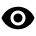
\includegraphics[height=10pt]{./images/iconos/ic_visibility_black_18dp.png}
        \UCpaso [\UCsist] accede a la pantalla \hyperref[fig:IU17]{IU17 Información del proyecto}. \label{item:CU17Item1} \Trayref{A}.
	\end{UCtrayectoria}

%--------------------------------------		
		\begin{UCtrayectoriaA}{A}{ El actor da click en el boton 'regresar'}
			\UCpaso [\UCsist] accde a la pantalla \hyperref[fig:IU09]{IU09 Gestionar Proyectos}.
		\end{UCtrayectoriaA}		
		
		
%-------------------------------------- TERMINA descripción del caso de uso.
%======================================================================================
\begin{UseCase}{CU18}{Eliminar proyecto}{
		Permite al Lider de proyecto eliminar un proyecto.
	}
		\UCitem{Actor}{\hyperlink{LiderProyecto}{Lider de proyecto}}
		\UCitem{Propósito}{Permitír al Lider de proyecto eliminar un proyecto}
		\UCitem{Entradas}{\begin{itemize}
		\item Ninguna 
		\end{itemize}
}
		\UCitem{Salidas}{Proyecto: eliminacion del proyecto}
		\UCitem{Destino}{Pantalla de gestión de proyectos}
		\UCitem{Precondiciones}{Que el proyecto no tenga tareas configuradas}
		\UCitem{Postcondiciones}{proyecto eliminado}
		\UCitem{Errores}{\begin{itemize}
		\item El proyecto no se puede eliminar, tiene tareas generadas.
		\end{itemize}}
		\UCitem{Observaciones}{}
	\end{UseCase}
%--------------------------------------
	\begin{UCtrayectoria}{Principal}
		\UCpaso[\UCactor] Da click en el icono 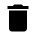
\includegraphics[height=10pt]{./images/iconos/ic_delete_black_18dp.png}
        \UCpaso [\UCsist] muestra diálogo con el mensaje '¿Desea eliminar el proyecto seleccionado?'.
        \UCpaso [\UCactor] Da click en el botón sí. \Trayref{A}
        \UCpaso [\UCsist] Verifica que no existan tareas creadas para el proyecto.\Trayref{B}
	\end{UCtrayectoria}

%--------------------------------------		
		\begin{UCtrayectoriaA}{A}{ El actor da click en el boton 'No'}
			\UCpaso [\UCsist] Cierra el cuadro de diálogo.
		\end{UCtrayectoriaA}
		
%--------------------------------------
		\begin{UCtrayectoriaA}{B}{ El proyecto tiene tareas generadas}
			\UCpaso [\UCsist] Cierra el cuadro de diálogo.
			\UCpaso [\UCsist] Muestra el mensaje \MSGref{MSG7}{El proyecto tiene tareas generadas}
		\end{UCtrayectoriaA}		
		
		
%-------------------------------------- TERMINA descripción del caso de uso.
%====================================================================================
\begin{UseCase}{CU19}{Registrar repositorio proyecto}{
		Permite al Lider de proyecto dar de alta el reositorio git en donde esten trabajando.
	}
		\UCitem{Actor}{\hyperlink{LiderProyecto}{Lider de proyecto}}
		\UCitem{Propósito}{Permitír al Lider de proyecto registrar el repositorio gt en donde estan versionando el proyecto.}
		\UCitem{Entradas}{\begin{itemize}
		\item URL Repositorio: url del repositorio donde esta el proyecto
		\item Usuario: nombre del usuario del repositorio
		\item Token: token que identifiacara el repositorio donde se la aloja el proyecto. 
		\end{itemize}
}
		\UCitem{Salidas}{Repositorio: registro del repositorio git del proyecto.}
		\UCitem{Destino}{Pantalla de gestión de proyectos}
		\UCitem{Precondiciones}{Que el proyecto no tenga tareas configuradas}
		\UCitem{Postcondiciones}{proyecto eliminado}
		\UCitem{Errores}{\begin{itemize}
		\item El proyecto no se puede eliminar, tiene tareas generadas.
		\end{itemize}}
		\UCitem{Observaciones}{}
	\end{UseCase}
%--------------------------------------
	\begin{UCtrayectoria}{Principal}
		\UCpaso[\UCactor] Da click en el icono 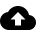
\includegraphics[height=10pt]{./images/iconos/ic_cloud_upload_black_18dp.png}
        \UCpaso [\UCsist] accede a la pantalla \hyperref[fig:IU19]{IU19 Registrar repositorio proyecto}.
        \UCpaso [\UCactor] introduce los campos obligatorios.
        \UCpaso [\UCactor] da click en el botón 'aceptar'.
        \UCpaso [\UCsist] Verifica que no se hayan omitido campo.         \label{item:CU19Item1}  \Trayref{A}
        \UCpaso Muestra mensaje de operecion exitosa.
	\end{UCtrayectoria}

%--------------------------------------		
		\begin{UCtrayectoriaA}{A}{ El actor no ingreso los datos requeridos}
			\UCpaso Muestra mensaje de falta de datos requeridos
			\UCpaso Continua en el paso \ref{item:CU19Item1} del \UCref{CU19}.
		\end{UCtrayectoriaA}
		
		
%-------------------------------------- TERMINA descripción del caso de uso.
% \IUref{IUAdmPS}{Administrar Planta de Selección}
% \IUref{IUModPS}{Modificar Planta de Selección}
% \IUref{IUEliPS}{Eliminar Planta de Selección}

% 


% Copie este bloque por cada caso de uso:
%-------------------------------------- COMIENZA descripción del caso de uso.

%\begin{UseCase}[archivo de imágen]{UCX}{Nombre del Caso de uso}{
%--------------------------------------
	\begin{UseCase}{CU09}{Ver Proyectos }{
    	Permite a un usuario ver los proyectos en los que participa como líder y como colaborador.
	}
		\UCitem{Actor}{\hyperlink{Líder de Proyecto, Colaborador.}{Líder de proyecto, Colaborador.}}
		\UCitem{Propósito}{Visualiza todos los proyectos en el que el actor participa.}
		\UCitem{Entradas}{\begin{itemize}
		\item Usuario: lo obtiene el sistema
		\end{itemize}
}
		\UCitem{Salidas}{Proyectos: los obtiene el sistema
}
		\UCitem{Destino}{Mis Proyectos.}
		\UCitem{Precondiciones}{Tener una cuenta creada, haber iniciado sesión, tener participación en proyectos.
}
		\UCitem{Postcondiciones}{Muestra todos los proyectos.
 }
		\UCitem{Errores}{}
		\UCitem{Observaciones}{}
	\end{UseCase}
%--------------------------------------
	\begin{UCtrayectoria}{Principal}
      \UCpaso  Muestra la pantalla principal.
		\UCpaso[\UCactor]Da click en la menú de mis proyectos
      \UCpaso  Muestra los proyectos en forma de lista.
	\end{UCtrayectoria}
        
		
%-------------------------------------- TERMINA descripción del caso de uso.